\documentclass[11pt,a4paper]{article}
\usepackage[margin=25mm]{geometry}
\usepackage{amsmath,amssymb,amsthm}
\usepackage{booktabs,multirow,longtable}
\usepackage{graphicx}
\usepackage{microtype}
\usepackage{hyperref}
\usepackage{enumitem}
\usepackage[T1]{fontenc}
\usepackage{lmodern}
\hypersetup{colorlinks=true,urlcolor=blue,linkcolor=blue,citecolor=blue}
\graphicspath{{../figures/}}
\renewcommand{\topfraction}{0.9}
\renewcommand{\bottomfraction}{0.8}
\renewcommand{\textfraction}{0.08}
\renewcommand{\floatpagefraction}{0.85}
\newcommand{\Q}{\mathbb{Q}}
\newcommand{\ZZ}{\mathbb{Z}}
\newcommand{\Reg}{\operatorname{Reg}}
\newcommand{\F}{\mathcal{F}}
\newcommand{\Cl}{\operatorname{Cl}_2}
\title{A Reproducible Census of Rank-Two Mordell--Weil Lattice Shapes\\for Elliptic Curves of Conductor Below 50,000}
\author{Toni Mladenovski\\\small Independent researcher\\\small ORCID: \href{https://orcid.org/0009-0009-8343-662X}{0009-0009-8343-662X}}
\date{23 November 2026\\\small v0.3.4 PREPRINT --- not peer reviewed}
\begin{document}
\maketitle
\begin{abstract}
We report a reproducible finite-population computation of canonical-height lattice shapes for all 23,612 elliptic-curve records of stated algebraic rank two and conductor $N<50{,}000$ in a pinned version of Cremona's \texttt{ecdata}. Alongside equal weighting of curves, we study 18,886 predetermined representatives, one per isogeny class. For a reduced height Gram matrix $G=\bigl(\begin{smallmatrix}h_1&b\\b&h_2\end{smallmatrix}\bigr)$, the dimensionless shape factor is $s=1-b^2/(h_1h_2)$. Its means are $0.953758660887$ (all curves) and $0.954750262395$ (class representatives), below the normalized hyperbolic reference mean $(3/\pi)\Cl(\pi/3)=0.969197841658$. The fractions with fundamental-domain height $y\ge2$ are $0.209512$ and $0.226729$, compared with the reference $3/(2\pi)=0.477465$. All supplied generator pairs already satisfy Gauss-reduction inequalities. Exact rational point checks and requested 192/256-bit PARI computations accompany the per-curve data. An AI-assisted rerun of the same pipeline and PARI engine in a separate environment matched all compared scientific fields across the 23,612 records. Additional same-engine comparisons, serialization effects and inherited database assumptions are distinguished from independent height algorithms or certified error bounds. The contribution is a pinned, reproducible census and a comparison of two fixed weighting choices. The results are descriptive observations on a bounded arithmetic population, without an asymptotic distribution claim or a BSD proof.
\end{abstract}
\noindent\textbf{Keywords:} elliptic curves; Mordell--Weil groups; canonical height; regulator lattice; Gauss reduction; arithmetic data; reproducible computation.\\
\textbf{MSC 2020:} 11G05, 11G50; 11Y40.

\section{Introduction}
The canonical-height pairing on the free part of the Mordell--Weil group of an elliptic curve $E/\Q$ defines a Euclidean lattice. For a basis of $E(\Q)/E(\Q)_{\rm tors}$ its Gram determinant is the regulator, while its shape after scaling is encoded by a point in a modular fundamental domain. Such shapes have been studied before: notably, Watkins examined rank-two Mordell--Weil lattice distributions in \S6.4 of \emph{Some heuristics about elliptic curves} \cite{Watkins2008}. His construction (shortest vector normalized to $1$, second generator moved into the $\mathrm{SL}_2(\ZZ)$ fundamental domain and reflected into $0\le x\le\frac12$) is the one used here, and his large prime-conductor sample exhibited a discrepancy with the hyperbolic reference measure. It does not follow that every different conductor-bounded census must follow the same distribution.

Our aim is limited and reproducible: describe the exact finite set of curves and representative-selection rule, calculate its rank-two lattice-shape statistics, and make the distinctions between stored output, reproduced numerical output, and mathematical proof explicit. The procedures build on standard height calculations and binary-form reduction \cite{Cohen1993,Cremona1997,PARI}. We claim neither a new BSD identity nor a new equidistribution theorem. We compare two fixed weighting schemes because enumerating isogenous models and enumerating classes are not the same statistical operation.

\section{Fixed data populations and mathematical quantities}
\subsection{Source data and selection}
Our source is the five \texttt{allgens} blocks for conductors below $50{,}000$ from J. E. Cremona's public \texttt{ecdata} repository \cite{CremonaData}, pinned to Git commit
\begin{center}\small\texttt{25cec5ecfec8b9f016eb1631ac633194c2bed39f}.\end{center}
A source record gives the conductor, Cremona class and curve number, Weierstrass $a$-invariants, stated rank, torsion structure, and generator coordinates. We parse projective triples $[X:Y:Z]$ with $Z\ne0$ as affine $(X/Z,Y/Z)$, not as $(X/Z^2,Y/Z^3)$; this distinction was checked by exact substitution. The rank and the spanning property of the supplied generator pairs are accepted from the pinned database rather than reproved here.

\begin{enumerate}[leftmargin=*]
\item \textbf{Population A (curve-weighted):} all 23,612 records with stated rank $2$ and $N<50{,}000$.
\item \textbf{Population B (class-weighted):} one predetermined record for each pair (conductor, isogeny-class code), selecting the smallest numerical Cremona curve number. This produces 18,886 classes; in every class the selected record is curve number~$1$. Cremona's documentation states that, for all $N$ up to $370{,}000$, curve~$1$ is the $\Gamma_0(N)$-optimal curve except in class 990h \cite{CremonaDocs}, and 990h has rank one, so it is not in this population. We rely on that documented statement and did not recompute optimality. Selecting one curve per class removes the multiplicity of isogenous curves but not every arithmetic dependence between classes.
\end{enumerate}
All five source blocks have recorded SHA-256 values, reproduced in the V0.2 package. The population-B selection file is fixed before any heights were computed.

\subsection{Gram matrices and the shape parameter}
For free generators $P,Q\in E(\Q)$, let $\langle\cdot,\cdot\rangle$ be the canonical-height bilinear pairing. Define
\begin{equation}
G=\begin{pmatrix}h_1&b\\b&h_2\end{pmatrix},\qquad h_1=\hat h(P),\quad h_2=\hat h(Q),\quad b=\langle P,Q\rangle,
\end{equation}
so that $\det G=h_1h_2-b^2>0$ for independent $P,Q$. If $\{P,Q\}$ spans $E(\Q)/E(\Q)_{\rm tors}$ then $\det G=\Reg(E)$; for a subgroup of index $d$ one would instead have $\det G=d^2\Reg(E)$. The spanning property is taken from \texttt{ecdata} (Section~\ref{sec:calc}). For a Gauss-reduced basis, the inequalities $0\le2|b|\le h_1\le h_2$ hold. Define
\begin{equation}
 x=\frac{|b|}{h_1}\in[0,1/2],\qquad y=\frac{\sqrt{\det G}}{h_1}>0,\qquad
 s=\sin^2\theta_{\rm red}=1-\frac{b^2}{h_1h_2}=\frac{y^2}{x^2+y^2}.
 \label{eq:shape}
\end{equation}
Since $x^2+y^2=h_2/h_1\ge1$, the coordinates lie in the folded fundamental domain $0\le x\le1/2$, $x^2+y^2\ge1$, and
\begin{equation}
 s=\frac{y^2}{x^2+y^2}\ \ge\ 1-\frac{1}{4(x^2+y^2)}\ \ge\ \frac34,
 \label{eq:bound}
\end{equation}
with equality if and only if $h_1=h_2=2|b|$ (the hexagonal lattice). Equivalently, $b^2/(h_1h_2)\le h_1/(4h_2)\le\frac14$. The determinant is invariant under every change of basis in $\mathrm{GL}_2(\ZZ)$; the unreduced angle is not. Every $\mathrm{GL}_2(\ZZ)$-class of positive-definite binary forms contains a reduced form whose triple $(h_1,h_2,|b|)$ is uniquely determined \cite{Cohen1993}. The reduced basis and its matrix $U$ need not be unique: simultaneous negation already gives the same Gram matrix, and boundary cases ($h_1=h_2$ or $2|b|=h_1$) admit additional choices. Thus $x$, $y$ and $s$ are invariants of the Mordell--Weil lattice up to isometry, and they are unchanged by rescaling the height normalization. They are \emph{not} invariants of the isogeny class: isogenous curves can have different normalized height-lattice shapes, so curve-weighted and class-weighted statistics need not agree. In the present population the smallest relative reduction margins were $(h_1-2|b|)/h_1=3.2\cdot10^{-5}$ and $(h_2-h_1)/h_2=3.3\cdot10^{-6}$, so both reduction margins were positive at the declared precision.

\subsection{Reference measure and correct normalization}
We compare these finite data to the normalized hyperbolic measure
\begin{equation}
 d\mu=\frac{6}{\pi}\frac{dx\,dy}{y^2},\qquad (x,y)\in\F_{+}=\{0\le x\le\tfrac12,\ x^2+y^2\ge1,\ y>0\}.
\end{equation}
On the folded domain the mean of $s$ is
\begin{equation}
 \mathbb E_{\mu}[s]
 =\frac6\pi\int_0^{1/2}\frac{\arcsin x}{x}\,dx
 =\frac3\pi\Cl(\pi/3)
 =0.969197841658351542\ldots,
 \label{eq:haarmean}
\end{equation}
where $\Cl(\phi)=\sum_{n\ge1}\sin(n\phi)/n^2$ denotes Clausen's function. The second moment is
\begin{equation}
 \mathbb E_{\mu}[s^2]=\tfrac12\mathbb E_{\mu}[s]+\tfrac14+\frac{3\sqrt3}{8\pi}=0.941347256612347789\ldots.
\end{equation}
For $Y\ge1$, the separate reference tail probability is
\begin{equation}
 \Pr_{\mu}(y\ge Y)=\frac3{\pi Y}.
 \label{eq:haartail}
\end{equation}
On the full domain $\{|x|\le\frac12,\ x^2+y^2\ge1,\ y>0\}$ the normalized measure is $(3/\pi)\,dx\,dy/y^2$; since $s$ and $y$ are even in $x$, all reference values above are the same for either normalization. Thus $3/\pi\simeq0.954930$ is a \emph{tail probability for $y\ge1$}, not the mean of $s$. For $3/4\le t<1$, direct integration gives the reference distribution function
\begin{equation}
 F_s(t)=\frac6\pi\left[\frac\pi6-\arcsin\sqrt{1-t}
 -\sqrt{\frac{1-t}{t}}\log\frac{1}{2\sqrt{1-t}}\right].
 \label{eq:cdf}
\end{equation}
The endpoint extension is $F_s(t)=0$ for $t\le3/4$ and $F_s(t)=1$ for $t\ge1$. The reference median, solving $F_s(t)=\frac12$, is $0.990015001853\ldots$. The reference is a comparison model; the finite arithmetic population is not presumed to be distributed according to it.

\section{Calculation and numerical verification}\label{sec:calc}
The public \texttt{ecdata} inputs were parsed with exact rational arithmetic. For each curve, both given free points and any torsion generators were checked to satisfy the original Weierstrass equation. There were 47,224 free-generator checks and 7,816 torsion-generator checks, with no failures. Heights were computed with \texttt{ellheightmatrix} using PARI/GP 2.19.1 through cypari2 2.2.9. The calculations were requested at 192 and 256 bits with explicit precision on the relevant method calls and fresh curve initialization. A complete record was retained for each curve; core numerical fields ($G$, $G_{\rm red}$, $\det G$, $x$, $y$, $s$) were serialized to 45 significant decimal digits, reduction margins to about 12 and precision-difference diagnostics to about 6. Differences between the precision runs provide a \emph{stability diagnostic}, not a mathematically certified error bound.

An integer transformation $U$ was tracked in the Gauss reduction. Tests included $\det U=\pm1$, $G_{\rm red}\approx U^{T}GU$, preservation of determinant, recomputed height matrices from transformed points, positive definiteness, and reduction inequalities. Because $U=I$ for every supplied basis (see below), the transformation identities alone do not exercise nontrivial reduction on the production data. Positive definiteness and the reduction inequalities remain substantive checks. Three sheared-basis controls per curve (bases $M(P,Q)$ with $\det M=1$, rebuilt from points) tested nontrivial reductions. The supplied Cremona bases were already reduced: $U=I$ in all 23,612 principal records. As a result, the experiment measures the shapes of the supplied reduced lattices; it does not show a distortion being removed from initially uncorrected Cremona bases.

The V0.2 software repaired four error-handling issues in its V0.1 predecessor: normalization at vanishing or nearly vanishing pairings, retry conditions for changing $U$, retention of failed-precision and missing-record information, and invalid export signaling. The prescribed run reported 67 self-tests, 7 negative controls, and 11 integration tests passing; deliberately injected failures produced the intended nonzero subprocess exit codes.

The verification evidence has three distinct scopes. First, Kimi re-executed the released pipeline in a separate environment with PARI/GP 2.19.1 and reported zero mismatches in the compared scientific fields across all 23,612 records. This was a reproduction using the same pipeline code and height engine. Second, Kimi used a separately written direct-\texttt{gp} calculation and reduction for 47 selected curves. Reanalysis of its saved output reported a maximum relative difference of approximately $4.6067\cdot10^{-45}$ against stored 45-digit fields, attained by the determinant of 18330t1. Third, Claude reported a different-call-path check of the raw Gram entries for all 23,612 curves, using \texttt{localbitprec(320)}, with maximum relative difference approximately $4.9733\cdot10^{-45}$ at $h_1$ for 38251a1. The latter check was performed by the pipeline's author. The two maxima refer to different populations and fields, and their relative-error denominators also differ; they are not repeated estimates of a single statistic.

All these height calculations use PARI's implementation. Their differences are consistent with rounding to 45 significant decimal digits, whose rounding contribution alone is bounded by $5\cdot10^{-45}$ relative to a nonzero unrounded value when rounding to nearest. This is not a certified bound on the error of the computed heights. No independently implemented second height engine or interval certification was used; choosing another front end would not establish independence without identifying its backend. An earlier direct comparison of the actual V0.1 and V0.2 archives reported no differences in the compared core fields and common summary fields. This is field equality, not byte identity of complete output files. The manuscript reviews did not document a new direct V0.1--V0.2 comparison; Kimi explicitly marked this check as not executed because the original V0.1 archive was unavailable in that review. Reviewer scripts, outputs and their limitations are recorded in the accompanying reconciliation report. No human specialist peer review has yet been obtained.

\section{Results}
\subsection{Overall population and reference comparison}
\begin{table}[htbp]\centering\small
\caption{The two fixed finite populations and hyperbolic comparison. Fractions for $y\ge Y$ are descriptive. Numbers are rounded for display.}\label{tab:main}
\begin{tabular}{lrrr}\toprule
Quantity&A: curves&B: class reps.&Reference $\mu$\\\midrule
Count&23,612&18,886&---\\
Mean $s$&0.953758661&0.954750262&0.969197842\\
Median $s$&0.971300150&0.972534735&0.990015002\\
Second moment $\mathbb E[s^2]$&0.912037434&0.913914839&0.941347257\\
Fraction $y\ge1$&0.932492&0.934661&0.954930\\
Fraction $y\ge2$&0.209512&0.226729&0.477465\\
Fraction $y\ge4$&0.019355&0.023139&0.238732\\
Fraction $y\ge8$&1/23,612&1/18,886&0.119366\\
Fraction $y\ge16$&0&0&0.059683\\
Maximum ECDF distance (descriptive)&0.216998&0.206008&---\\\bottomrule
\end{tabular}
\end{table}
The ECDF distance is $D_n=\sup_t|F_n(t)-F_s(t)|$, where $F_n(t)=n^{-1}\#\{i:s_i\le t\}$. It is evaluated at both sides of each observed jump; for sorted observations $s_{(i)}$ this is
\[
D_n=\max_{1\le i\le n}\max\left\{\frac{i}{n}-F_s(s_{(i)}),\ F_s(s_{(i)})-\frac{i-1}{n}\right\}.
\]
The mean $s$ in A is $0.01543918\ldots$ below the reference mean, and that in B is $0.01444758\ldots$ below it. The upper $y$ tail is substantially shorter than the reference in both populations: only 457 curves in A and 437 representatives in B have $y\ge4$, while exactly one record in either population has $y\ge8$. As the populations are deterministically defined and curves in A may be isogenous, these descriptive distances are not IID sampling tests; no p-values or asymptotic inference are assigned.

\begin{figure}[htbp]\centering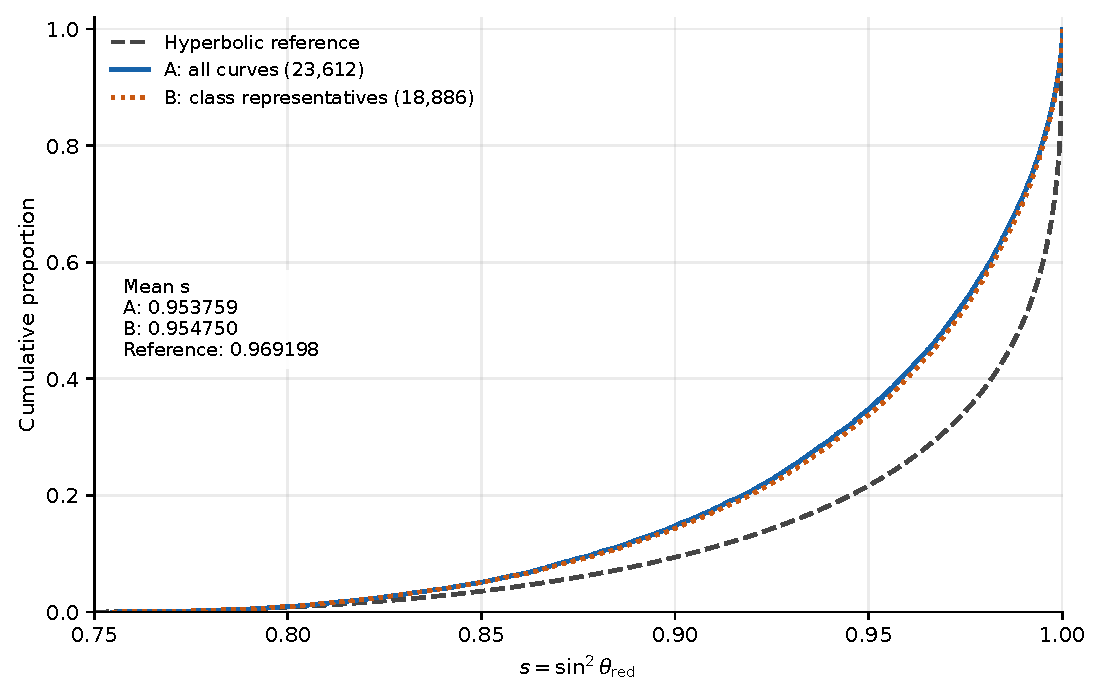
\includegraphics[width=0.94\linewidth]{fig1_ecdf_s_vs_reference.pdf}\caption{Empirical cumulative distributions of $s$ for the two fixed populations and the hyperbolic reference. The curves are not independent random draws from the reference.}\label{fig:ecdf}\end{figure}
\begin{figure}[htbp]\centering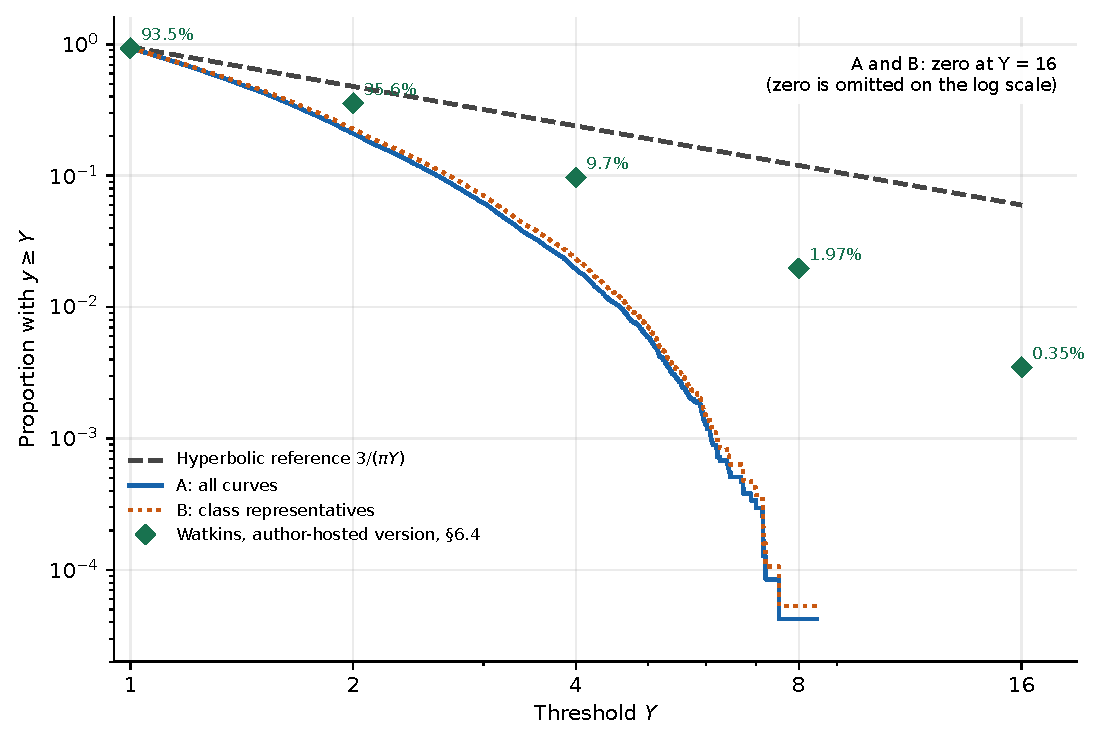
\includegraphics[width=0.94\linewidth]{fig2_y_tail.pdf}\caption{Observed tails of the reduced fundamental-domain coordinate $y$ versus the hyperbolic reference $3/(\pi Y)$. Diamonds: the author-hosted version of Watkins's paper \cite[\S6.4]{WatkinsAuthor}, for its distinct prime-conductor population. Its percentages differ from arXiv v2 \cite{WatkinsArxiv}; the source versions are kept separate. Both present populations have zero records with $y\ge16$, which cannot be displayed on the logarithmic vertical axis.}\label{fig:tail}\end{figure}
\subsection{Conductor blocks and class weighting}
\begin{table}[htbp]\centering\small
\caption{Means of $s$ and fractions with $y\ge2$ by conductor block (reference: $0.969198$ and $3/(2\pi)=0.477465$).}\label{tab:blocks}
\begin{tabular}{lrrrrrr}\toprule
Conductor range&$n_A$&Mean $s_A$&$y\ge2$ (A)&$n_B$&Mean $s_B$&$y\ge2$ (B)\\\midrule
1--9,999&2,388&0.954460&0.232412&1,969&0.955396&0.243271\\
10,000--19,999&4,410&0.953301&0.214286&3,490&0.954801&0.235244\\
20,000--29,999&5,212&0.953402&0.212011&4,183&0.954465&0.229978\\
30,000--39,999&5,671&0.953662&0.197849&4,517&0.955176&0.214523\\
40,000--49,999&5,931&0.954222&0.205699&4,727&0.954289&0.222340\\\midrule
Total&23,612&0.953759&0.209512&18,886&0.954750&0.226729\\\bottomrule
\end{tabular}
\end{table}
All ten block-by-population means lie below the reference mean. There is no visible monotone convergence across these five blocks, but the narrow and low-conductor range cannot resolve asymptotic behavior. The two weighting schemes yield similar mean $s$ but not interchangeable distributions: the fraction with $y\ge2$ shifts from $20.9512\%$ to $22.6729\%$, a difference of $1.7217$ percentage points.

\begin{figure}[htbp]\centering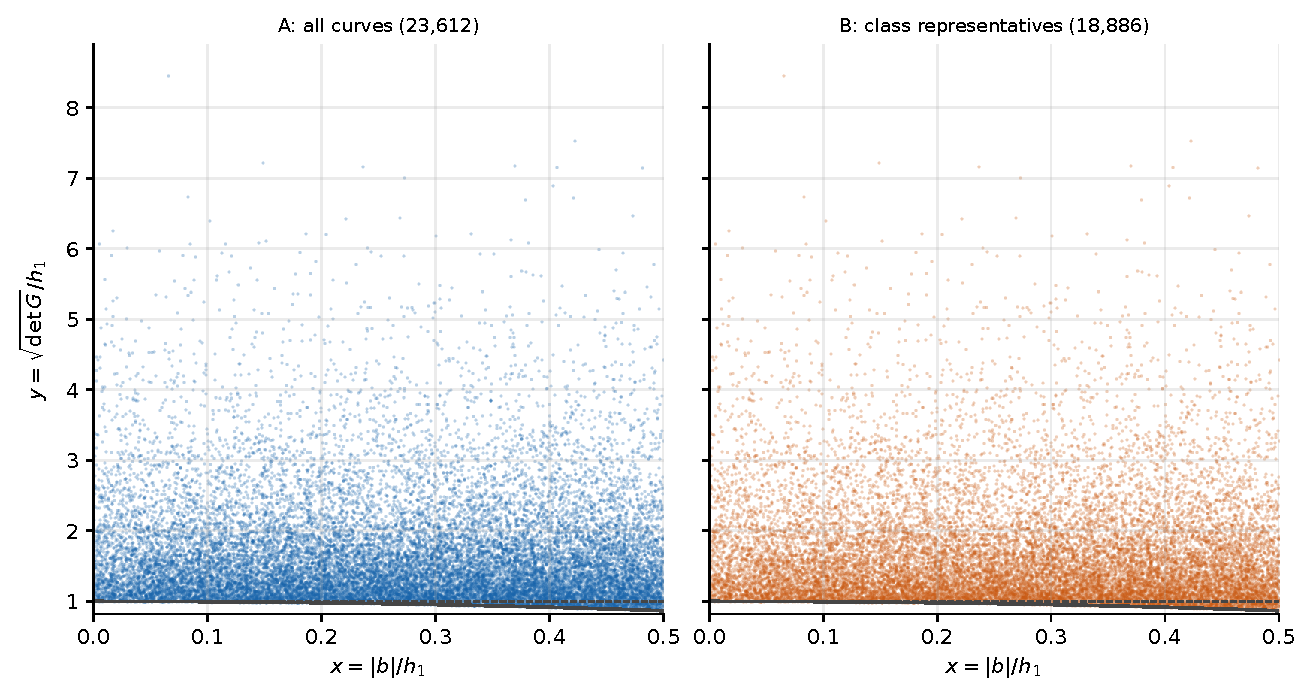
\includegraphics[width=0.94\linewidth]{fig3_fundamental_domain.pdf}\caption{The recorded folded-domain coordinates $(x,y)$ for the two populations. Source figures were generated from the finite census.}\label{fig:domain}\end{figure}

\subsection{Relation to earlier literature}
Watkins \cite[\S6.4]{WatkinsAuthor,WatkinsArxiv} studied a different set: all 2,143,079 curves of analytic rank two and prime conductor below $10^{10}$ in the Stein--Watkins database. For 2,114,188 of them \texttt{mwrank} provably determined the Mordell--Weil group, and further descent methods reduced the remaining cases to 54. He reported approximately $93.5\%$ with $y\ge1$, against $(1/2)/(\pi/6)\approx95.5\%$ under Haar measure. He also found a non-uniform distribution in $x$ for $y\ge1$, and $y$ tails that are heavier than ours but lighter than the reference. The tail percentages differ between arXiv v2 \cite{WatkinsArxiv} (35.4, 9.4, 1.7 and 0.2\% for $y\ge2,4,8,16$) and the author-hosted version \cite{WatkinsAuthor} (35.6, 9.7, 1.97 and 0.35\%); Figure~\ref{fig:tail} explicitly uses the latter. These are source-version observations; we do not identify either set as the journal printing without inspecting that printing. Watkins himself left open whether the discrepancy reflects the small-discriminant selection of his data or an incorrect Haar hypothesis. The near-agreement of our class-weighted fraction $0.934661$ with his quoted $93.5\%$ does not imply the same underlying population, selection mechanism, or limiting law. We cannot attribute the observed differences uniquely to conductor cutoff, isogeny weighting, or the arithmetic of canonical heights.

\section{Scope, limitations and research implications}
The computations are a deterministic census conditional on the supplied \texttt{ecdata} rank and generator claims. Neither PARI rerunning nor exact point substitution independently proves every generator set is a saturated basis. A single height engine was used throughout; an independently implemented second engine and/or certified interval methods would strengthen numerical error control. The 192/256-bit comparison measures stability without proving interval bounds. The present work does not establish a limiting measure as $N\to\infty$, does not reject a probabilistic model at a specified significance level, and does not prove the BSD conjecture or the full order of any Tate--Shafarevich group.

Within these limits, the delivered data provide a reproducible comparison of two specific conductor-bounded weighting choices. Future work could extend the conductor cutoff and analyze lower bounds on canonical heights, regulator size, discriminant sign, and isogeny-class stratification to investigate the shortened $y$ tail. A larger, methodologically distinct computation is necessary before attributing the departure to an asymptotic arithmetic phenomenon.

\section*{Data and code availability}
The V0.2 data and code are currently preserved as the ZIP archive\begin{center}\footnotesize\texttt{BSD\_MW\_SHAPE\_STUDY\_V0\_2.zip}\end{center}with SHA-256
\begin{center}\footnotesize\texttt{1338bdf8ddb50de5d9278a14e207ee3c3f2c9ab211d929b3556d7adf92a0d4fc}.\end{center}
The corresponding unchanged V0.1 archive has SHA-256
\begin{center}\footnotesize\texttt{ce2a7de2585b87996acc13b404fb36680631c6b93aef473c0d8499307b273d55}.\end{center}
The package includes pinned sources and hashes, exact point checks, test logs, per-curve results and figures. The dataset record for Study~V0.2 is identified by \href{https://doi.org/10.5281/zenodo.24484435}{doi:10.5281/zenodo.24484435}; this preprint is identified by \href{https://doi.org/10.5281/zenodo.24484370}{doi:10.5281/zenodo.24484370}. The accompanying \href{https://github.com/eit-orbitos/BSD_MW_RANK2_SHAPE_CENSUS_50000}{GitHub source repository} contains the reproducible code, selected stored summaries and manuscript sources. Redistributed \texttt{ecdata} inputs retain Artistic License~2.0 \cite{CremonaData}; the supplement supplies the unchanged upstream license, README and attribution. The author's original software is under \href{https://polyformproject.org/licenses/noncommercial/1.0.0}{PolyForm Noncommercial~1.0.0}. The original manuscript, figures and documentation, and any author-held licensable rights in the original result compilation, are under Creative Commons Attribution--NonCommercial~4.0 International (\href{https://creativecommons.org/licenses/by-nc/4.0/}{CC BY-NC~4.0}). Separately attributed third-party material is excluded from those grants. The older BSD calculator release v3.15.4 is a separate work; its DOI does not identify this census.

\section*{AI assistance, authorship and verification disclosure}
ChatGPT (OpenAI) assisted with manuscript organization and drafting from author-supplied material. Claude (Anthropic) developed and executed the V0.1/V0.2 study pipeline and repairs, including PARI calculations. Kimi (Moonshot AI) reran V0.2 and checked its output; ChatGPT checked files, summaries and V0.1--V0.2 archive consistency. Kimi and Claude reviewed manuscript v0.3, and Claude proposed v0.3.1. ChatGPT reconciled those reviews, checked input hashes, and recomputed stored-data summaries and reference quantities; no new PARI heights were computed in that reconciliation. Claude's software review shares authorship with the pipeline; the rerun and direct-GP checks share the PARI height engine. These are AI-assisted technical checks, not human peer review. Toni Mladenovski is the sole human author and retains responsibility for the manuscript and conclusions. No AI system is listed as an author.

\section*{Author declarations}
\noindent\textbf{Funding.} This research received no external funding or grants.

\noindent\textbf{Competing interests.} The author declares no competing interests.

\noindent\textbf{Research provenance.} The author conducted the study as an independent researcher using publicly available data and literature, together with internally developed research notes and study-specific definitions. Established mathematical definitions and results remain attributed to their sources. The AI assistance described above remains part of the provenance.

\begin{thebibliography}{9}\small\setlength{\itemsep}{1pt}
\bibitem{Watkins2008} M. Watkins, \emph{Some heuristics about elliptic curves}, Experimental Mathematics \textbf{17} (2008), no.~1, 105--125, doi:\href{https://doi.org/10.1080/10586458.2008.10129019}{10.1080/10586458.2008.10129019}; \href{https://arxiv.org/abs/math/0608766}{arXiv:math/0608766}, \S6.4.
\bibitem{WatkinsAuthor} M. Watkins, \emph{Some heuristics about elliptic curves}, author-hosted manuscript, \S6.4, \url{https://magma.maths.usyd.edu.au/~watkins/papers/heur.pdf} (accessed 23 November 2026; source hash recorded in the supplement). This is the source of the historical markers in Figure~\ref{fig:tail}.
\bibitem{WatkinsArxiv} M. Watkins, \emph{Some heuristics about elliptic curves}, \href{https://arxiv.org/abs/math/0608766v2}{arXiv:math/0608766v2}, 30 August 2006, \S6.4.
\bibitem{Cohen1993} H. Cohen, \emph{A Course in Computational Algebraic Number Theory}, Graduate Texts in Mathematics 138, Springer, 1993.
\bibitem{Cremona1997} J. E. Cremona, \emph{Algorithms for Modular Elliptic Curves}, second ed., Cambridge University Press, 1997.
\bibitem{CremonaData} J. E. Cremona, \emph{Elliptic Curve Data} (\texttt{ecdata}), GitHub repository, pinned commit \texttt{25cec5ecfec8b9f016eb1631ac633194c2bed39f}, Artistic License 2.0, \url{https://github.com/JohnCremona/ecdata}; release record doi:10.5281/zenodo.161341 (accessed 23 November 2026).
\bibitem{CremonaDocs} J. E. Cremona, \emph{The elliptic curve database for conductors to 500000}, documentation of \texttt{ecdata}, \url{https://johncremona.github.io/ecdata/} (accessed 23 November 2026).
\bibitem{PARI} The PARI Group, \emph{PARI/GP} version 2.19.1 (\texttt{ellheight} uses the normalization of \cite{Cremona1997}), documentation and source, \url{https://pari.math.u-bordeaux.fr/} (accessed 23 November 2026).
\end{thebibliography}
\end{document}
